\section{Modelling concept\label{sec:model_concept}}

\subsection{Model type}
\par{
    The central model concept is the use of a 2D \acrfull{cnn} to provide 3D segmentation masks, trained on point annotated data.
    Out-of-the-box pre-trained 2D networks are available, with weights pre-trained on public datasets\footnote{\label{footnote:Imagenet}For example, weights trained on the ImageNet dataset. 
    This dataset consists of over $14.10^6$ images of more than $2.10^4$ categories.}.
    An alternative approach would be to use 3D networks, which is a logical choice for volumetric data, with the apparent advantage that the 3D convolution layers naturally take into account the volumetric structure of the data.
    One could argue that using 2D networks deprives the network of crucial \textit{context} information in the direction perpendicular to the slice it is analysing (this work tries to meet this issue in section \ref{section:twoDplus} on page \pageref{section:twoDplus}).     
}

However, there are advantages to choosing 2D networks over 3D networks:
\begin{enumerate}
    \item Since the number of parameters (weights) to train scales exponentially with the kernel dimension, the number of parameters to train is considerably higher for a 3D \acrshort{cnn} compared to a corresponding 2D \acrshort{cnn}.
    \item The academic community has investigated 2D \acrlong{cnn}s for several years. The networks can be initialised with weights pre-trained on vast and diverse datasets (see remark \ref{footnote:Imagenet} on ImageNet). 
    These datasets indeed do not contain the specific classes nor the specific datatype investigated in this project. 
    However, the different convolution layers have proven to extract useful general features that allow the network to distinguish an extensive range of categories. 
    These features have proven to be sufficiently general to apply to new machine vision applications. This practice is called transfer learning.
    \item Although consecutive slices are strongly correlated, there is more data\footnote{There are more slices than volume segments in 1 image volume.} to train the networks, certainly when considered in proportion to the number of weights to be trained.
\end{enumerate}

\subsection{Model training approach}

An approach used often in weakly supervised learning is the generation of \textit{ersatz} or \textit{pseudo} mask labels\cite{Laradji2019,Laradji2019a, Ahn2019,McEver2020}, see page \pageref{sec:PreviousWork_weaklySupervised}.
This project intends to use this approach too.

A scan volume can be sliced along 3 different axes: the transverse axis, the coronal axis and the sagittal axis (see figure \ref{fig:anatomicalPlains}), meaning that 3 different models can be trained with the available point annotated data. 
Each of these 3 networks will have different context elements to segment the sliced images.
The resulting segmentation volumes\footnote{The segmentation results of a stack of 2D slices can be combined to form a 3D segmentation volume.} of these three networks can then be combined to obtain a final segmentation volume.
This final segmentation mask, which should be as least as good as the best of the 3 individual model results, can then be used as pseudo masks to train a final \textit{fully supervised} network. 

\begin{SCfigure}[][htb]
    \centering
    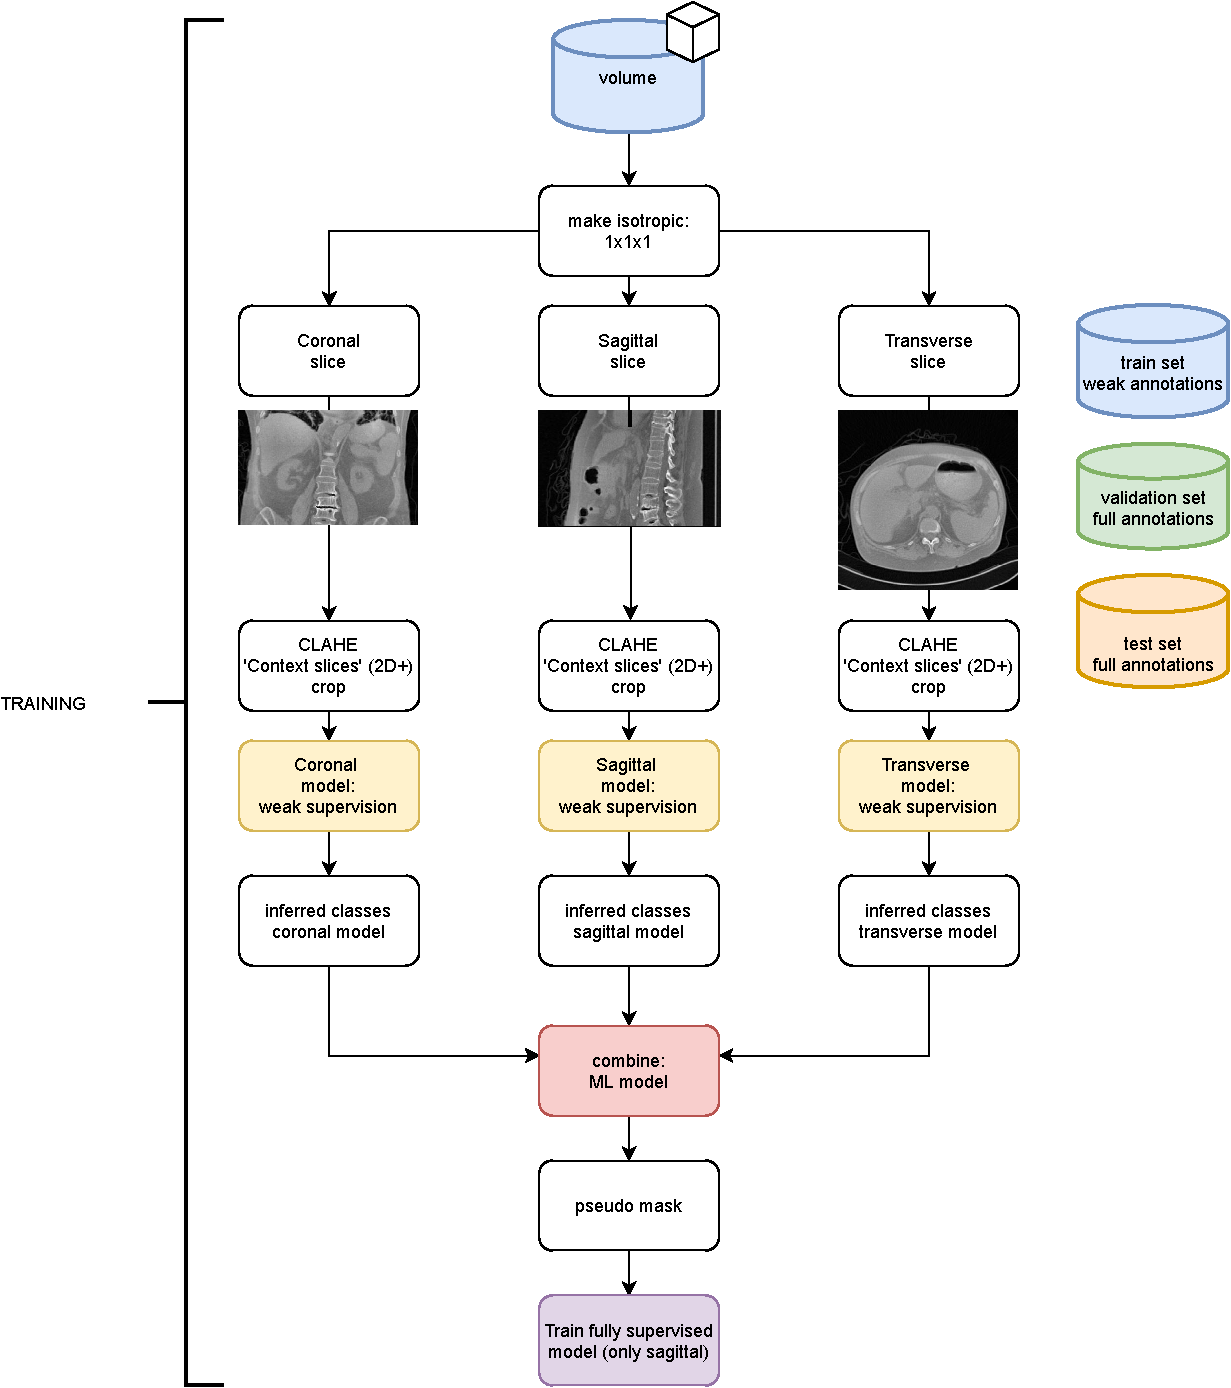
\includegraphics[width=.95\textwidth]{/home/thesis/images/Training_concept.pdf}
    \caption{\label{fig:model_training_concept}Illustration of the model training approach. 
    This is based on the conbination of 3 different models based on different volume slices.}
\end{SCfigure}

When the segmentation masks of a new, unknown volume need to be inferred, only this final model must be evaluated.
Only one set of slices along a single dimension needs to be generated and preprocessed to perform this evaluation.

\begin{SCfigure}[][htb]
    \centering
    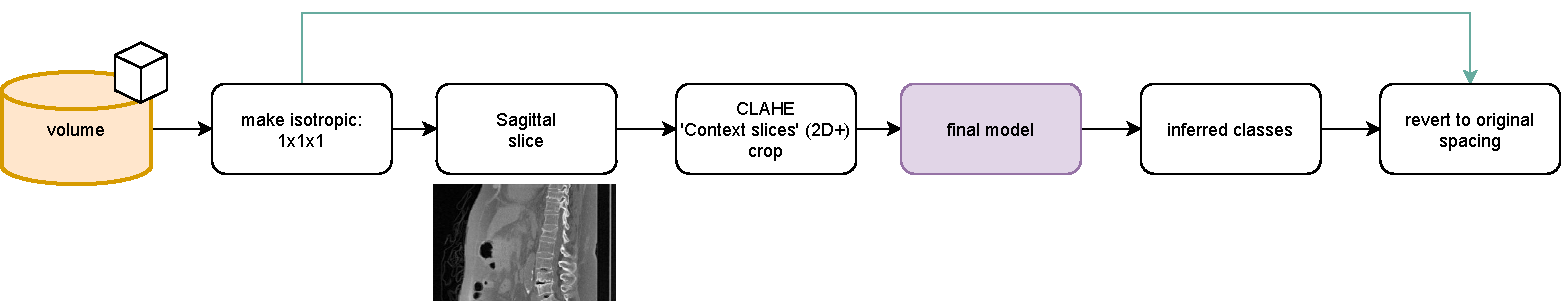
\includegraphics[width=.95\textwidth]{/home/thesis/images/Inference_concept.pdf}
    \caption{Inference step. Only one model needs to be evaluated in this step, the model that is trianed in the final step of the training procedure illustrated in figure \ref{fig:model_training_concept}.}
\end{SCfigure}

\section{Volume combination procedure\label{sec:combinationProcedure}}
To construct one pseudo mask volume, three single dimension models are first evaluated to form three stacks of two-dimensional estimated segmentation masks, and the obtained results are combined to form three segmentation volumes. 
The resulting set of three segmentation volumes is then combined to form a new segmentation volume.
This last segmentation volume, made out of the combination, is sliced again to obtain the pseudo masks for the final model.
The procedure described here was only devised after observation of the single-dimensional model results.

\subsection{Recombination of the crops to slices}
All models are designed for $352 \times 352$ crops of the 2D slices\footnote{More information on the cropping of the slices can be found in chapter \ref{sec:cropping} on page \pageref{sec:cropping}.}.
To construct a segmentation volume from a single dimensional model, all relevant\footnote{Some slices have dimensions that do not allow to extract 5 different $352 \times 352$ crops. See for example figure \ref{fig:smallcrop} on page \pageref{fig:smallcrop}.} crops of each volume slice are evaluated.
First, the segmentation results on these crops have to be combined again to obtain a segmentation mask of the whole slice.
Due to the cropping procedure, different crops of the same slice always partly overlap.
The crops are combined by averaging the logits $z_i$ for the overlapping positions.
The inferred class is then obtained from the resulting average $z_i$ values for that position. 

\begin{SCfigure}[][htb]
\begin{minipage}{.99\textwidth}
    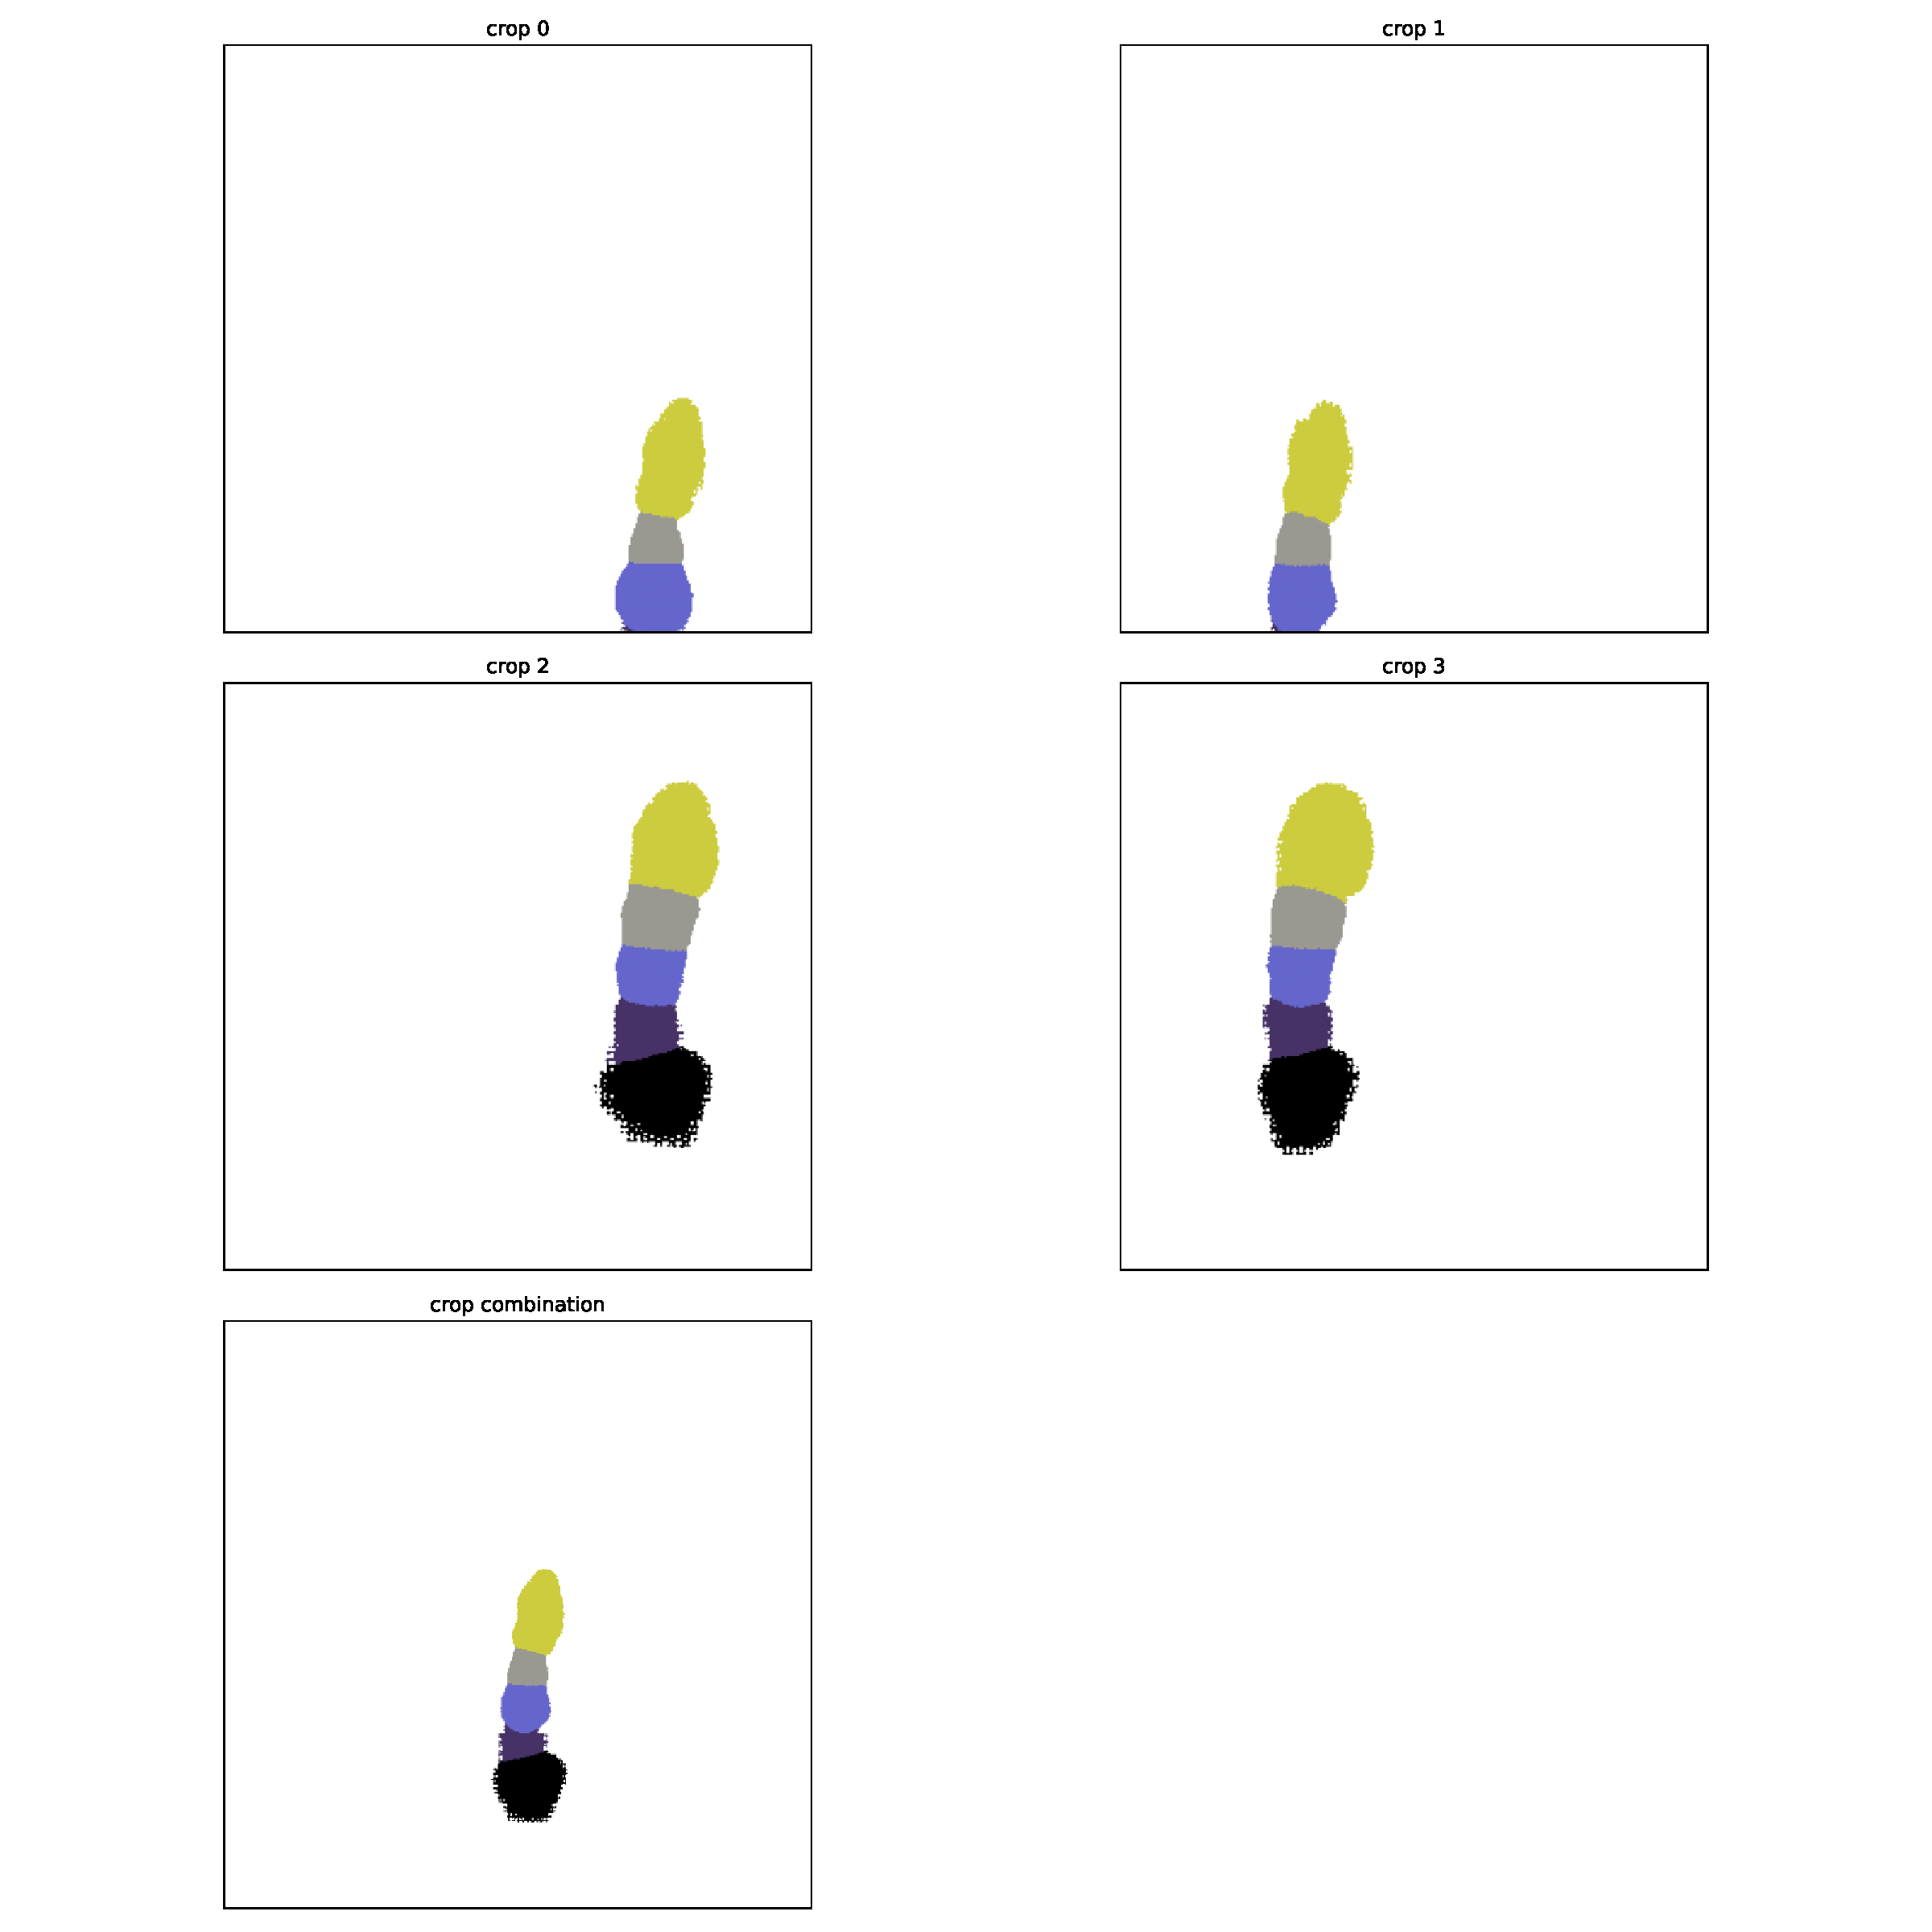
\includegraphics[width=0.95\textwidth]{images/USiegen_004_50_crops.pdf}
\end{minipage}
\begin{minipage}{.99\textwidth}
    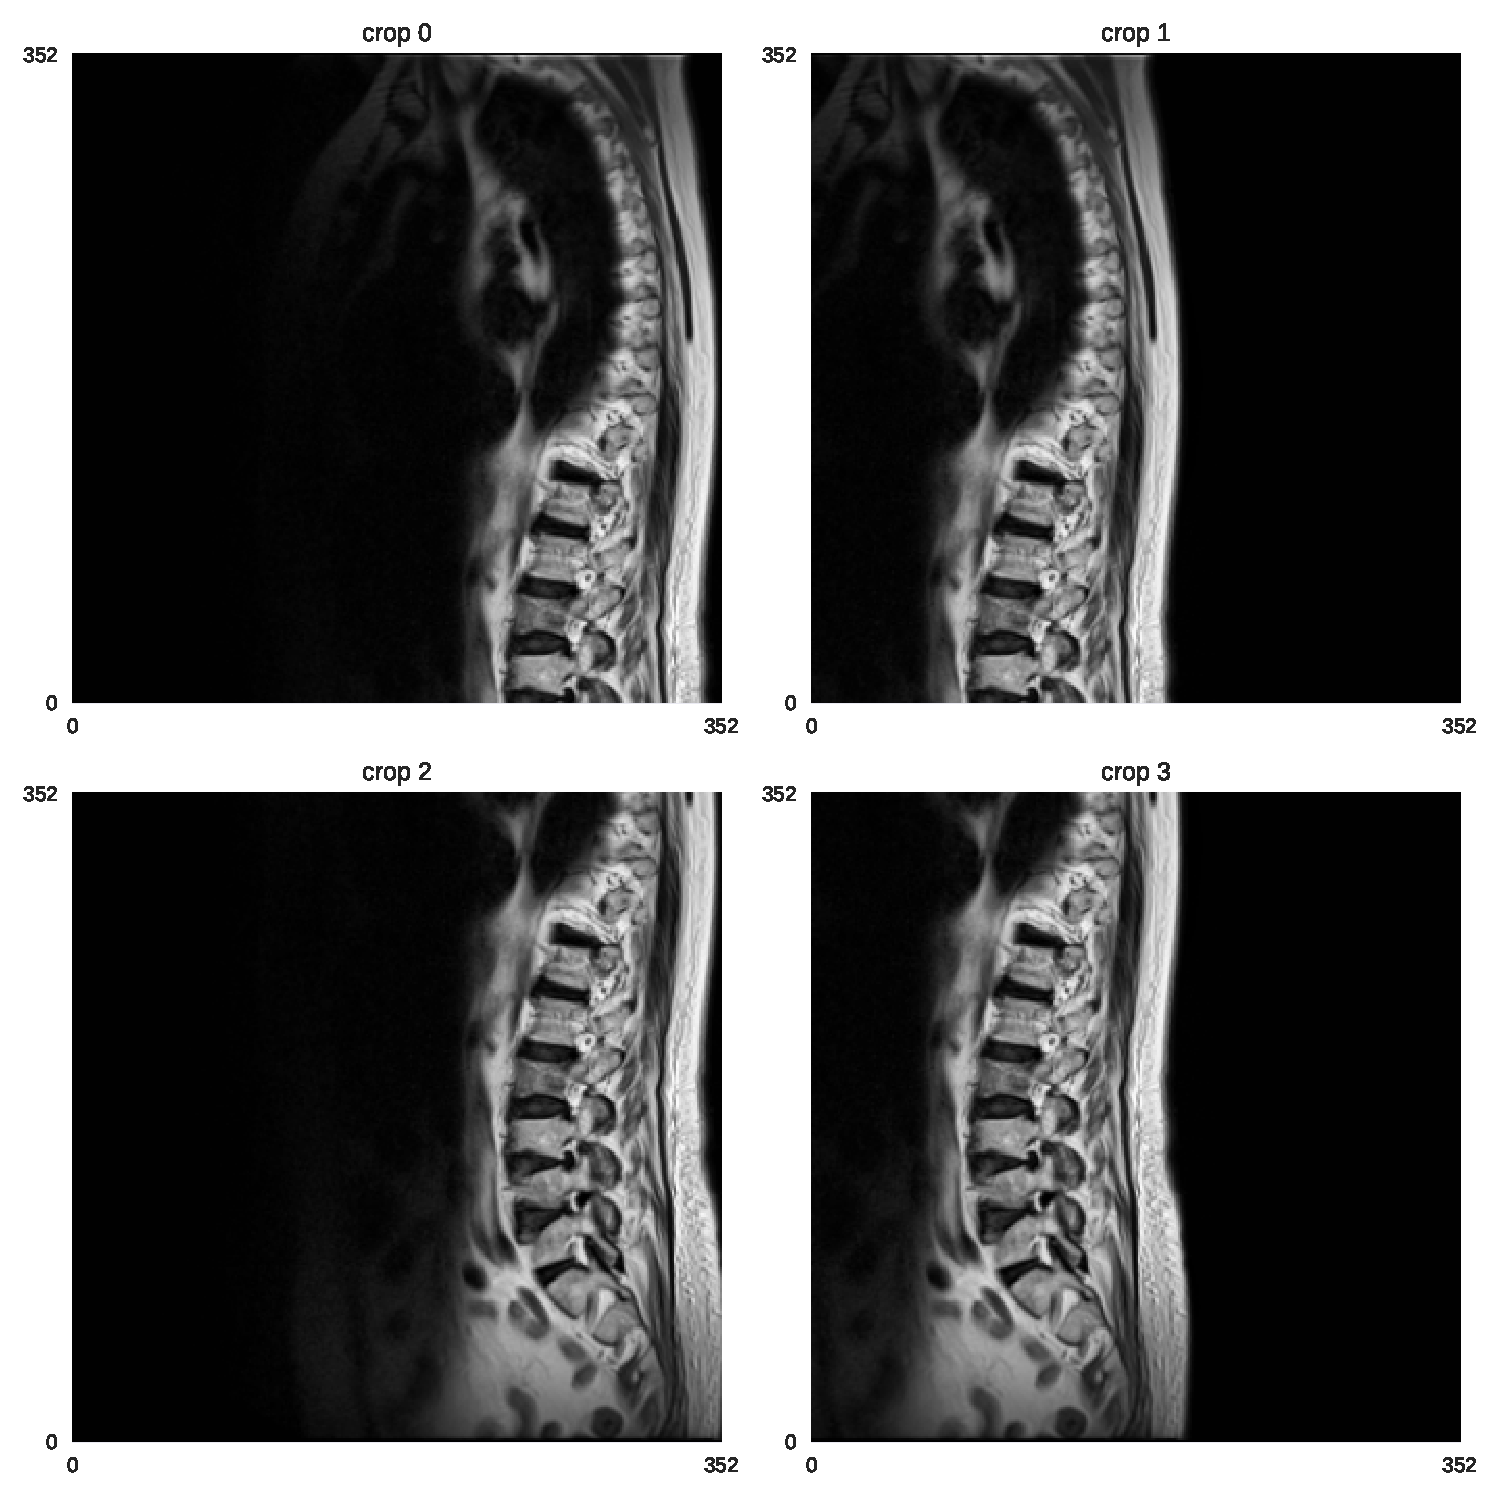
\includegraphics[width=0.95\textwidth]{images/cropping_slice050.pdf}
\end{minipage}
    \caption{Sagittal slice 50 of the USiegen 04 volume has to be evaluated in 4 crops due to its dimensions. The recombination of these crops to form the mask for the slice is illustrated in this figure. As a reference, the corresponding images are provided.}
\end{SCfigure}

\subsection{Rule based result combination}
Once a stack of class segmentation masks for all volume slices are obtained, these can be combined to form a segmentation volume.
Combining the results of three different single dimension models is performed in two steps:
\begin{enumerate}
    \item The resulting classification volumes are first combined with a rule-based method.
    \item After this rule-based combination, the resulting segmentation estimation is smoothened with a morphological filter.
\end{enumerate}

Three single dimension models are trained:
\begin{description}
    \item[Transverse slices] offer little context to indicate which of the lumbar vertebrae they contain. 
    It does not seem easy even for a human expert to indicate which vertebra is visible on the slice.
    The model trained on these slices is intended only for semantic segmentation.
    For each pixel is inferred only if it represents a vertebra, without distinction between the different lumbar vertebrae. 
    \item[Sagittal \& Coronal slices] do offer the necessary context to distinguish between $L_1$ to $L_5$. 
    The models trained on these slices do indicate the specific lumbar vertebra index. 
\end{description}

The volume combination rules are based on two observations:
\begin{enumerate}
    \item The precision (see equation \ref{eq:precision_i} on page \pageref{eq:precision_i}) with which the background class is predicted in all models is very high.\newline
            This means $\mathcal{P} \left( label = background \mid prediction = background \right)$ is high for all models. 
            If one model indicates a position is background, this position could be estimated to be background with high probability.
    \item All models tend to overestimate the extent of the vertebrae, which causes a low recall score. The direction in which the predictions tend to \textit{bleed out} is different for the different models. 
\end{enumerate}
The observations mentioned above can be combined in algorithm \ref{alg:combination}.

\subsection{Morphological smoothing}
After the rule-based combination of estimations from different single dimension models, the result is smoothened with standard morphological filters.
These filters are combinations of the morphological \textit{erosion} and \textit{dilation} operators\footnote{
    This document is not intended to provide an elaborate explanation on morphological operations.
    For the readers conventience, the following symbolic notations are repeated:
    \begin{description}
        \item[Erosion] of set $\mathbf{A}$ by structural element $\mathbf{B}$ : $\mathbf{A} \ominus \mathbf{B}$ 
        \item[Dilation] of set $\mathbf{A}$ by structural element $\mathbf{B}$ : $\mathbf{A} \oplus \mathbf{B}$ 
        \item[Opening] of set $\mathbf{A}$ by structural element $\mathbf{B}$ : $\mathbf{A} \circ \mathbf{B} = (\mathbf{A} \ominus \mathbf{B}) \oplus \mathbf{B}$
        \item[Closing] of set $\mathbf{A}$ by structural element $\mathbf{B}$ : $\mathbf{A} \bullet \mathbf{B} = (\mathbf{A} \oplus \mathbf{B}) \ominus \mathbf{B}$
    \end{description}
}.
\par{
    Noise in the single dimension segmentation masks is suppressed with an opening operation on the individual segmentation volumes of the single dimension models.
    Noise in the combined volumes is suppressed by first opening and then closing the volumes.
    The estimated volumes are observed to overestimate the extent of the vertebrae. For this reason, an erosion step is performed to decrease the overall extent of the class masks.
}
\par{
    The procedure mentioned above has two hyperparameters: the number of iterations for the denoising filters and the number of iterations for the erosion filter.
    Both hyperparameters are estimated by calculating the same evaluation metric, the weighted dice score on the validation set, as for the single-dimensional model evaluation. 
    
    The combination of the rules and morphological smoothing operations discussed above results in the following algorithm to combine the segmentation volumes from the single dimension models\footnote{
        The algorithm shown here is based on the two observations mentioned.
    }:
}
\begin{algorithm}[H]
    \SetAlgoLined
    \KwData{
        Results $y_.$ of three models indicating an estimated class for all positions $\vec{p}$ in the volume. \;
        Transverse model $y_t \in \mathbb{N}^3: \forall y_t(\vec{p}) \in \{ 0, 1 \}$ \;
        Sagittal model $y_s \in \mathbb{N}^3: \forall y_t(\vec{p}) \in \{ 0, 1, 2, 3, 4, 5 \}$ \;
        Coronal model $y_c \in \mathbb{N}^3: \forall y_t(\vec{p}) \in \{ 0, 1, 2, 3, 4, 5 \}$  \;
        Binary $\mathbf{B}$ structure with rank 3 and connectivity 3 \;
    }
    \KwResult{Combination of the three model results $y_f$.}
    \tcp{Closing operation on all $y_.$}
    $y_t \leftarrow y_t \bullet \mathbf{B}$ \;
    $y_s \leftarrow y_s \bullet \mathbf{B}$ \;
    $y_c \leftarrow y_c \bullet \mathbf{B}$ \;
    \For{all $\vec{p}$}{
        $i \in [ 1, 2, 3, 4, 5]$ \;
            \lIf{$y_t[\vec{p}] = 1 \wedge y_s[\vec{p}] = i \wedge y_c[\vec{p}] = i$}{
                $y_f[\vec{p}] \leftarrow i$ 
            }
            \lElse{
                $y_f[\vec{p}] \leftarrow 0$ 
            }
        }
    
    $y_f \leftarrow ((y_f \circ \mathbf{B}) \bullet \mathbf{B}) \ominus \mathbf{B}$
   \caption{Rule based combination of model results from three single dimension models\label{alg:combination}}
\end{algorithm}